\chapter{Methods}\label{ch:methods}
This chapter will cover the approach taken to implement HKED safeguards into the SSPM. An introduction to the ORIGEN modeling of spent fuel will be the first step, then an introduction to the MCNP model will be the second topic. This will be followed by methods used to decrease runtime and automate generation of the MCNP simulations.


\section{Used Fuel Source Terms}
Spent nuclear fuel is primarily composed of very lightly enriched uranium, with around 5\% fission products, and 1-2\% plutonium. However, burnup, length of operating cycles, downtimes between cycles, and original fuel enrichment, among other factors, can cause the isotopics of spent fuel to vary from one discharge to another. This implies that using a single spent fuel composition for HKED modeling could be misrepresentative, and lead to incorrect KED k-edge drops, for example. To rectify this, the first part of this project was to identify common spent fuel enrichments and burnups. This was based off of a Los Alamos National Laboratory empirical relationship [insert citation], relating burnup to original enrichment. 

It is beneficial to describe the ORNL SCALE code before continuing. SCALE is, among other things, a reactor physics code which includes multiple sub-packages. One of these packages is the Oak Ridge Isotope Generation (ORIGEN) code. This code solves the Bateman equations to handle depletion cases for nuclear fuel. This code allows researchers to predict discharge isotopic compositions based off of reactor power, cycle length, and downtimes. 

Once the space of enrichment and burnup values was determined, a Python script was written by Jonathan Mitchell and Steven Skutnik to automate production of ORIGAMI (an alternative input format to ORIGEN) input decks. A change that was made to this script by Michael Cooper was to switch the reactor cycle lengths and number of cycles from the original 12 months and 5 cycles, to the values of 18 months and 3 cycles. This change was based on the fact that the United States reactors typically operate on 18 month cycles [insert MIT and EPRI references]. The Python ORIGAMI generation script was then used to generate the ORIGEN input to use in the SCALE. 

\todo[inline,color=red!30]{\textbf{SES:} I'll provide you with an ORIGAMI citation.}

The range of burnups was restricted to the low point of 20 GWd/MTU, and high point of 60 GWd/MTU. This were chosen based off of typical US spent fuel composition, assuming an average burnup of 45 GWd/MTU. Fuel rods on the edges of reactors will not have as high of burnup due to reactor operators optimizing the reactor neutronics, and could have values significantly lower than the average 45 GWd/MTU. Values below 20 GWd/MTU are typically reserved for special cases such as research reactors or weapons material generation [insert weapons reference]. Values above 60 GWd/MTU typically don't occur in the US due to the fuel generating neutron poisons over time and depleting the U-235 in the fuel. 

With this in mind, the enrichment and burnup values chosen for the spent fuel source terms are listed in Tables \ref{source1} and \ref{source2}. 

\todo[inline,color=red!30]{\textbf{SES:} Let's talk about possibly reformatting this table or using a longtable; there's really no reason for this to be two separate tables.}
\begin{table}[p!]
\caption{Spent Fuel Compositions For Source Terms}
\label{source1}
\begin{center}
\begin{tabular}[b]{|c|c|c|}
	\hline
	Burnup $\frac{GWd}{MTU}$ & Enrichment & Cooling Time (Years)\\ \hline
	20 & 1.96\% & 5 \\ \hline
	20 & 1.96\% & 15 \\ \hline
	20 & 2.17\% & 5 \\ \hline
	20 & 2.17\% & 15 \\ \hline
	20 & 2.39\% & 5 \\ \hline
	20 & 2.39\% & 15 \\ \hline
	25 & 2.26\% & 5 \\ \hline
	25 & 2.26\% & 15 \\ \hline
	25 & 2.51\% & 5 \\ \hline
	25 & 2.51\% & 15 \\ \hline
	25 & 2.76\% & 5 \\ \hline
	25 & 2.76\% & 15 \\ \hline
	30 & 2.55\% & 5 \\ \hline
	30 & 2.55\% & 15 \\ \hline
	30 & 2.83\% & 5 \\ \hline
	30 & 2.83\% & 15 \\ \hline
	30 & 3.11\% & 5 \\ \hline
	30 & 3.11\% & 15 \\ \hline
	35 & 2.81\% & 5 \\ \hline
	35 & 2.81\% & 15 \\ \hline
	35 & 3.13\% & 5 \\ \hline
	35 & 3.13\% & 15 \\ \hline
	35 & 3.44\% & 5 \\ \hline
	35 & 3.44\% & 15 \\ \hline


\end{tabular}
\end{center}
\end{table}



\begin{table}[p!]
\caption{Spent Fuel Compositions For Source Terms (continued)}
\label{source2}
\begin{center}
\begin{tabular}[b]{|c|c|c|}
	\hline
	Burnup $\frac{GWd}{MTU}$ & Enrichment & Cooling Time (Years)\\ \hline
	40 & 3.07\% & 5 \\ \hline
	40 & 3.07\% & 15 \\ \hline
	40 & 3.41\% & 5 \\ \hline
	40 & 3.41\% & 15 \\ \hline
	40 & 3.75\% & 5 \\ \hline
	40 & 3.75\% & 15 \\ \hline
	45 & 3.31\% & 5 \\ \hline
	45 & 3.31\% & 15 \\ \hline
	45 & 3.68\% & 5 \\ \hline
	45 & 3.68\% & 15 \\ \hline
	45 & 4.05\% & 5 \\ \hline
	45 & 4.05\% & 15 \\ \hline
	50 & 3.55\% & 5 \\ \hline
	50 & 3.55\% & 15 \\ \hline
	50 & 3.94\% & 5 \\ \hline
	50 & 3.94\% & 15 \\ \hline
	50 & 4.34\% & 5 \\ \hline
	50 & 4.34\% & 15 \\ \hline
	55 & 3.77\% & 5 \\ \hline
	55 & 3.77\% & 15 \\ \hline
	55 & 4.19\% & 5 \\ \hline
	55 & 4.19\% & 15 \\ \hline
	55 & 4.61\% & 5 \\ \hline
	55 & 4.61\% & 15 \\ \hline
	60 & 3.99\% & 5 \\ \hline
	60 & 3.99\% & 15 \\ \hline
	60 & 4.44\% & 5 \\ \hline
	60 & 4.44\% & 15 \\ \hline
	60 & 4.88\% & 5 \\ \hline
	60 & 4.88\% & 15 \\ \hline

\end{tabular}
\end{center}
\end{table}


Now that the source term generation has been described, a discussion of the HKED MCNP model is next. \\

\section{MCNP Modeling of HKED}

\subsection{MCNP Model}
A MCNP model was constructed by former UT PhD student Matt Cook as part of his dissertation project \cite{Cook2015}. This model contains the geometries needed to properly describe a HKED measurement apparatus such as the one shown in Figure \ref{HKED-apparatus}. This MCNP model works by performing two stage simulations for KED and XRF scenarios separately. Since the measurements are not interdependent, this allows for the KED and XRF to be handled separately for simulation, then the results can later be corroborated. This aids in the ease of building and troubleshooting the model.


\begin{figure}[h]
  \centering
  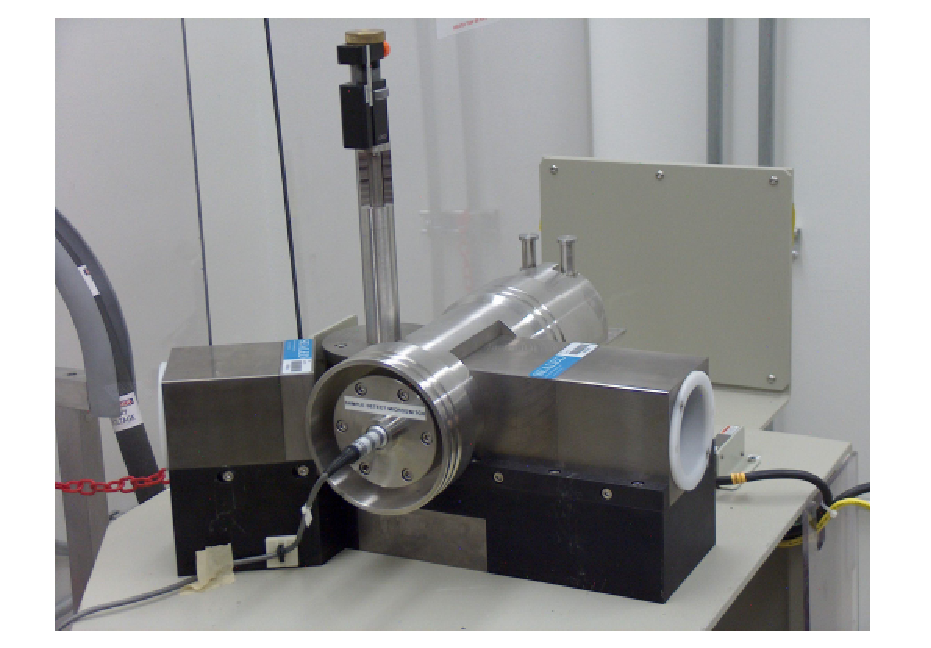
\includegraphics[width=15cm]{HKED_Apparatus.pdf}
  \caption{HKED system without outer lead shielding. Both XRF (left) and KED (right) component beamlines are exposed and germanium detectors have been removed \cite{Cook2015}}
 \label{HKED-apparatus}
\end{figure} 


When the model was received by Michael Cooper, there was minimal instruction on how to use the model.  The first step of this project was to recover the knowledge needed to run the MCNP model, as it had been over a year since it had been developed, and Matt Cook, the only person with intimate knowledge of using the model at the time, was working on a different task after his graduation. To this goal, the model was thoroughly reviewed, along with review of Cook's dissertation, to reveal the following method of operation. 

The model operates on several principles. The first is that the model uses 2 stages. The stage-1 simulations are used to generate gamma energy distributions exiting the beamline, which are to be used for the source file for the stage-2 simulations. The stage-2 simulations determine the pulse height response using F8 tallies. This effectively means that the stage-1 simulations guide the stage-2 simulations by building a more focused gamma source term  exiting the beamline that is going from the salt sample to the detector \cite{Cook2015}.  % last sentence needs reworded as it is a run-on

\subsection{Preliminary Work Performed On Model}

The first step that was done with the MCNP model to get it operating properly was to simply run it as is, and check the output. The first version of the model used was the KED version, as it was the easier of the two to converge statistically. The stage-1 model was ran, the results processed and a source term output generated, then the stage-2 ran. The output of the stage-2 pulse height tally, however, did not match the published results from Cook's dissertation, even when using an identical fuel/salt mixture. After discussion with Skutnik and Cook, it was realized that the Cd-109 source term that was used for normalization in Cook's dissertation results was not being included, due to using the incorrect version of the stage-1 postprocessing script. After the correct version was used (along with modifications to the script to properly reference the correct MCNP surfaces), a comparable pulse height spectra was obtained for the sample case of EBR fuel using the stage-2 simulation output. 

For the XRF version of the model, the first step again was to simply run the model as it was given. The results of the stage-2 XRF simulations, however, revealed a very jagged pulse height spectrum, with very high uncertainty. The next step was to inspect the stage-1 output, where it was realized that extremely few particles were actually reaching the F2 tally used to generate the gamma source term for the stage-2 simulation. Simulations were then ran increasing the number of stage-1 particles ran, but this did not make an appreciable difference in the number of particles reaching the F2 tally. Following this, a review was done of the variance reduction that was implemented in the model. It was determined that the DXTRAN variance reduction had been commented out in the model that was given, which resulted in extremely few particles reaching the F2 tally. To rectify this, the proper DXTRAN was turned on around the stage-1 F2 tally, and the model was run again. This time, the trial runs produced results that matched those published in Cook's dissertation \cite{Cook2015}. 

The overall variance reduction techniques employed in the XRF model were as follows \cite{Cook2015}:
%
\begin{enumerate}
\item \textbf{Forced collisions:} All particles entering the sample are required to interact and weighted appropriately
\item \textbf{MCNP DXTRAN Sphere:} Particles are forced to travel to the sphere volume, and are weighted appropriately
\item \textbf{Spatial weight window mesh:} Particles are weighted and controlled via splitting and Russian roulette based on position
\item \textbf{Energy weight window mesh:} Particles are weighted and controlled via splitting and Russian roulette based on energy
\end{enumerate}
%
\subsection{Generation of MCNP Outputs for Modeling}

It was determined that to properly model the k-edge drop and x-ray fluorescence peaks, a relatively large number of MCNP runs with acceptable statistical convergence would be needed. To accomplish this, 54 MCNP runs were done for the stage-1, and then 54 for the stage-2 simulations, with this being done for both KED and XRF. A total of 216 MCNP simulations were ran. These are based on \ref{source1} and \ref{source2}. 

The first step for the KED aspect of the MCNP model is to find the total mass fraction of actinides. Then using the Python script Convert\_Origen.py, the ORIGEN output is imported to Python. The elemental composition of the spent fuel source term from ORIGEN is determined in the form of mass percents. These mass percents are then proportionately assigned to the MCNP model's total mass percentage of fuel in the salt, replacing the default values of EBR spent fuel with commercial spent fuel mentioned in Tables \ref{source1} and \ref{source2}. Typical values of total fuel mass percent of the salt are around 7\%, with 6.8\% of the salt fuel mixture's mass percent being uranium, and plutonium making up the majority of the remainder. This convention of mass percents follows one of the two methods to specify to MCNP the percentage of elements in each material used in the model. Of note, for commercial spent fuel, there is an extremely small presence of any actinides other than uranium and plutonium, with uranium being vastly more abundant than plutonium. This will cause the plutonium k-edge drop to be barely visible.  % This needs reworded: it assumes the reader is familiar with MCNP mass percentage convention, and without MCNP knowledge, this paragraph isn't readable.

After the mass percentages of the materials in the MCNP input decks are corrected, the stage one simulations can be ran in sequence. This was done via batch scripting on a local computer built to handle moderately large MCNP tasks. A total of 250 million particles were ran for each stage-1 run, requiring approximately 2.5 hours per each simulation on an Intel Core i7-8700. The more particles that are ran, the better the stage-1 energy source file that is generated will be, however, increasing the number of particles increases runtime proportionately, while uncertainty is proportional to $\frac{1}{\sqrt{N}}$. This states that in order to reduce uncertainty by a factor of 10, the number of particles must be increased by a factor of 100. As such, there is an optimization between runtime and acceptable uncertainty. 

Once the 54 stage-1 simulations are complete, they are then put through a Python postprocessing script that Matt Cook wrote, to extract and write the energy source files to be used in the stage-2 simulations. The stage-2 simulations are then ran, again via batch script, to get the final detector response results that are desired. For the stage-2 simulations, 100 million particles are used, and the run time is typically around 2.5 hours. 

After the completion of the the stage-2 simulations are complete, the MCNP output file is then processed by the Python script \texttt{Spectra\_Retrieve.py}. This script searches the MCNP output for the F8 tally results, and converts them from the text file they are supplied in to a more usable .csv file. This facilitates importing of the spectra that were simulated into a Python script for empirically modeling the K-edge drop. 

A similar approach is followed for the XRF version of the model, however, the XRF requires significant variance reduction. Without multiple methods of variance reduction, the XRF version of the model requires trillions of particles to converge, with unrealistic runtimes. The variance reduction employed was described in the section on preliminary work with the model. 

\subsection{Potential Issues With MCNP Modeling}

The overall task of modeling HKED with MCNP works very well. However, due to MCNP's Monte Carlo nature, there are a few issues. The first is statistical uncertainty, and the second is ``particle hanging.'' % Note in LaTeX, smart quotes are ``blah'' 

For the HKED models, both KED and XRF, the uncertainty listed in the output of the S2 tally is not necessarily correct. This is because of the way the simulation works. The S1 simulation guides the particles to the entrances of the beamlines, where a F2 tally is waiting to generate a source term for the S2 simulation. Therefore, there is intrinsic uncertainty in the S2 source term, resulting from the S1 simulation results. In a sense, since the S1 simulations are guiding the S2 simulations, if the S1 simulation has an ultra large uncertainty, it can misguide the source term energy distribution used by the S2 simulations. This will not be reflected in the output of the S2 F8 tally, as it is only concerned with particles traveling from the beamline to the microcell target, without any care for how many particles actually reach the beamline. In reality, extremely few particles (on the order of typically less than 10) reach each energy channel for the S1 tally, causing extremely high variance. As a result, even though the S2 MCNP output will list uncertainties on the order of 1-5\% for KED, and less than 1\% for XRF, these values should be taken with a grain of salt, as they can be very misleading. However, with regards to reliability of the model to accurately reproduce HKED spectra, this is assumed to be true, based on benchmarking of HKED data done by Cook \cite{Cook2015}. As of now, the assumption will be that both the KED and XRF simulations model the spectra to within 5\% as the S2 results indicate. 

Regarding particle hanging, what is being referred to is an anomaly within Monte Carlo. Using Monte Carlo, it is theoretically possible for a particle to never terminate, and thus for a program such as MCNP to require infinite time to track a particular particle. This is extraordinary rare for normal MCNP simulations, however, when running simulations with extensive variance reduction and particle weighting modifications, it is possible. As such, in around 1 out of 50 simulations ran, the simulation would get stuck and hang on a particle. When this occurred, the solution was to simply redo the simulation run, as at most 1 day of simulation time was wasted. 




